%to do
\section{background}
\label{sec:background}
\subsection{cloud computing}
\begin{figure}
\centering
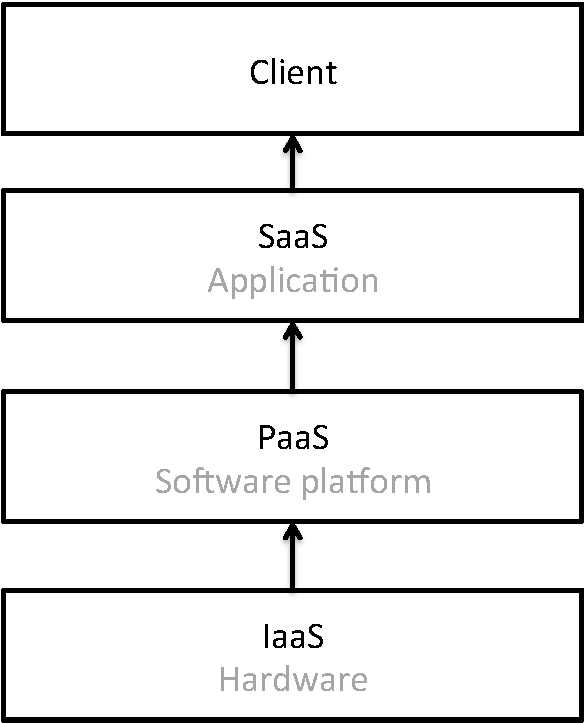
\includegraphics[width=4cm]{img/cloud_models.pdf}
\caption{the relationship of different cloud models}
\label{background:cloud models}
\end{figure}

Cloud computing refers to a model that cloud vendors provide user IT resources and charge them for
the resources they used.
Cloud vendors can offer hardware resources including CPU, memory, hard disk, network and software
resources OS, software suits and applications.
Cloud computing majorly can be classified into following three kinds of models:
\begin{enumerate}
  \item Infrastructure as a service (IaaS): cloud vendors provide only raw machines(physical or
  virtual machine), user need to set up the whole software environment including OS.
  \item Platform as a service (PaaS): in this model, cloud vendors provide hardware as well as
  software platform. Users can use it as a common computer and run applications on the platform.
  Amazon EC2 provides PaaS.
  \item Software as a service (SaaS): Cloud vendors provide a certain applications. Users don't need
  to configure the software themselves.
\end{enumerate}
The relationship of different cloud models can be shown as Figure~.\ref{background:cloud models}

Cloud computing can have following benefits:
\begin{itemize}
  \item User don't need to care about the machine placement and maintenance.
  \item User don't need a large number of machines to meet a temporally request peek and idle for
  the other time, Since cloud instances can set up in a few minutes when the request peek occurs.
  \item User don't need to pay for expensive hardware and software, they just need to pay for what
  they used.
\end{itemize}

\subsection{interconnection network in cloud}
\begin{figure}
\centering
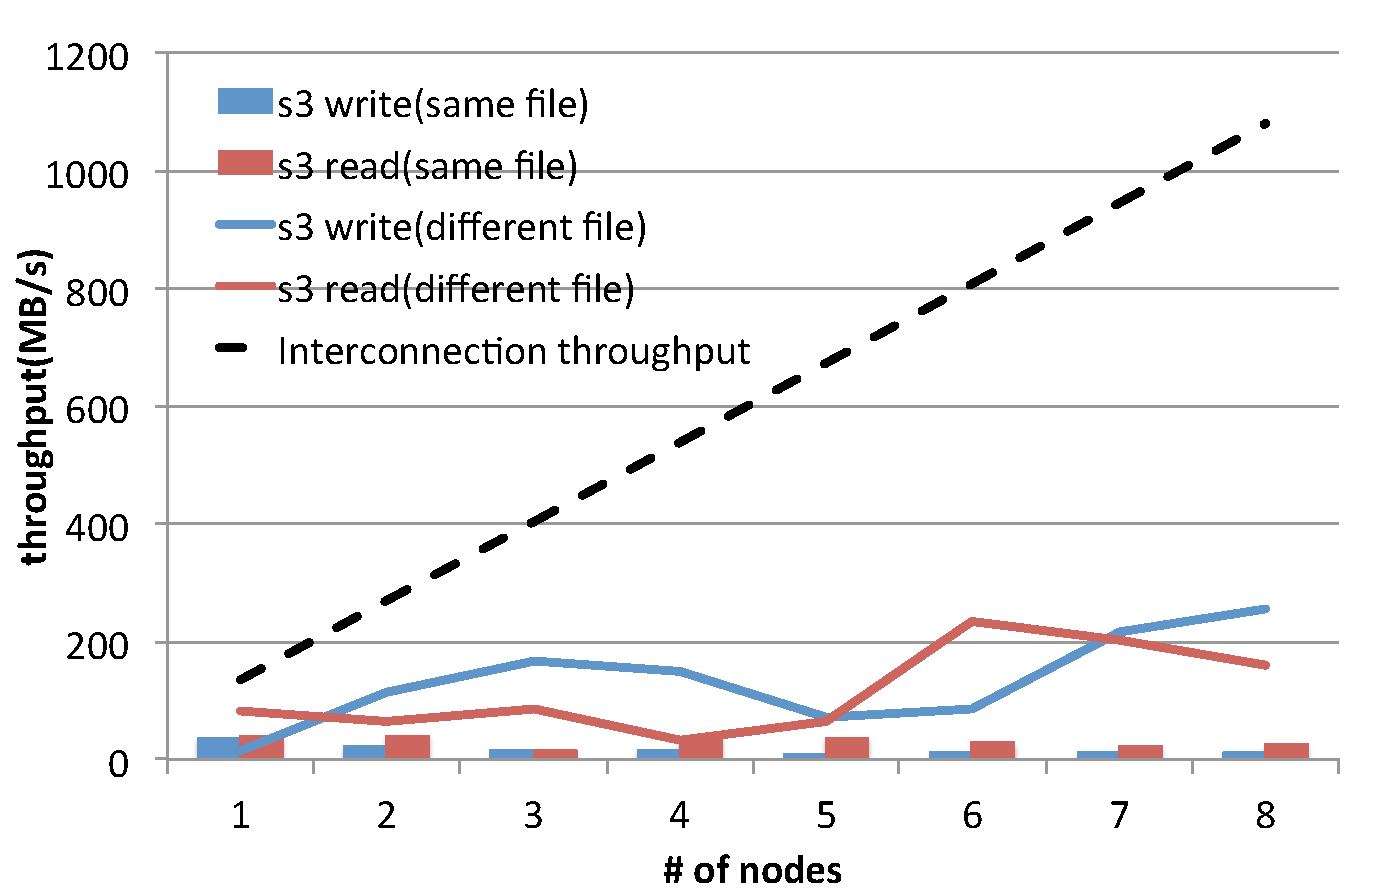
\includegraphics[width=8cm]{img/amazon_throughput}
\caption{Amazon Interconnection Network Throughput}
\label{}
\end{figure}

We use Iperf\cite{iperf}, which was developed by NLANR/DAST as a modern alternative for measuring
TCP and UDP bandwidth performance, and IOR\cite{IOR}, which is widely used for benchmarking
parallel file systems using POSIX, MPIIO, or HDF5 interfaces.

We can see that the I/O throughput also grows as number of nodes grows but the aggregate throughput
is only 100-140 MB/s, which is limited by Internet bandwidth, about 40-80 times smaller than
throughput inside TSUBAME.
For data-sensitive application, low I/O throughput is devastating, especially for application
running on supercomputers, furthermore, lower I/O throughput leads a longer execution time,
according to Amazon pay-as-you-go policy, longer execution time means more cost.

However, when we look at interconnection network throughput inside Amazon as Figure.~\ref{point to
point connection AMAZON} shows, although we only show the result up to 8 pairs of nodes, each node
achieved only 135MB/s (1GBit/s), the influence between nodes is extremely small, figure shows a
perfect linear line also a strong scalability.
since when we running the benchmark, many other users were also running applications on Amazon, so
we can assume that highest throughput 1GB/s (8Gbit/s) shown in Fig.~\ref{point to point connection
AMAZON} is not the maximum bandwidth of interconnection network in Amazon EC2 .
Comparing Fig.~\ref{point to point connection AMAZON} with Fig.~\ref{throughput AMAZON to OURLAB} 
and Fig.~\ref{point to point connection LAB}, interconnection network throughput is much higher than
Internet, it shows that our solution, by using I/O buffer nodes can achieve a higher
interconnection network throughput than Internet.
\subsection{burst buffer}
\begin{figure}
\centering
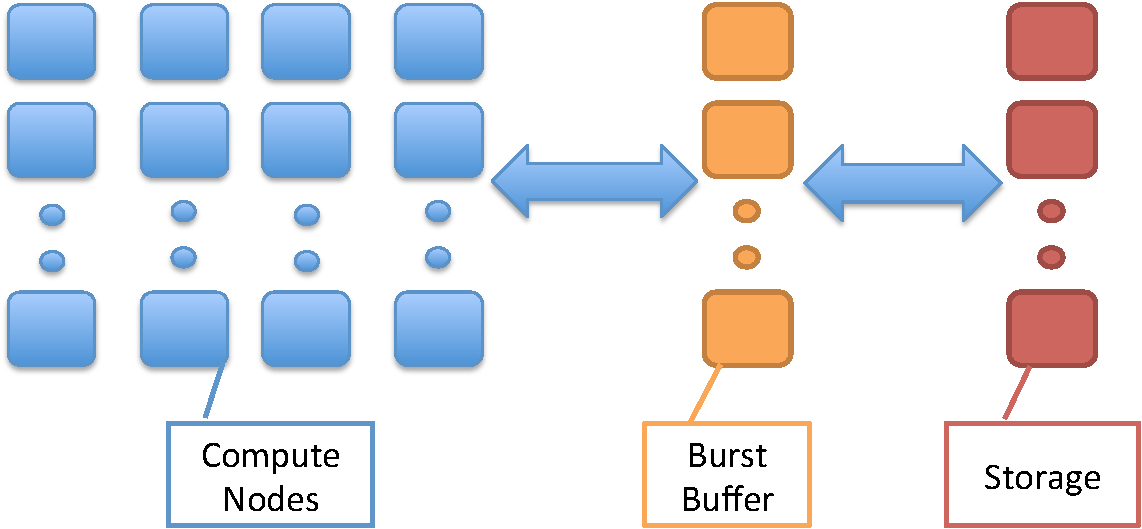
\includegraphics[width=8cm]{img/burst_buffer.pdf}
\caption{burst buffer architecture}
\label{background:burst buffer architecture}
\end{figure}

Modern high performance systems consist of thousands of compute nodes, and hundreds of
applications are running at the same time, some I/O request peak can hardly be meet by current
storage hierarchy. 
Traditional approach which solve such problem by providing a higher bandwidth storage will cause
the storage system underutilization.
Previous research\cite{on_the_role_of_burst_buffers} proposed a
burst buffer system as a new tier of current storage hierarchy.
Burst buffer system use several local compute nodes as a burst buffer to absorb I/O
request. 
By adding such new tier of storage hierarchy, temporilal I/O request can be absorb by burst buffer
without a need of a higher bandwidth storage. Figure~.\ref{background:burst buffer architecture}
shows the architecture of burst buffer.

Such burst buffer system can burst the application which has a high data locality I/O pattern, since
the data can be read once from storage and then buffered in the burst buffer system, subsequent
request for the same data can be accessed from burst buffer.
Furthermore, applications which write a lot also can benefit from burst buffer system, by buffering
output data in burst buffer, application can go ahead without waiting data be finally write to
storage.

\subsection{Data Locality}

\begin{table}
\centering
\begin{tabular}{|c|c|}
Montage		&		an application\\
pov ray\\
supernovae\xtq{not exact}
\end{tabular}
\caption{Work Flow Applications}
\label{background:work flow applications}
\end{table}

\begin{figure}
\centering
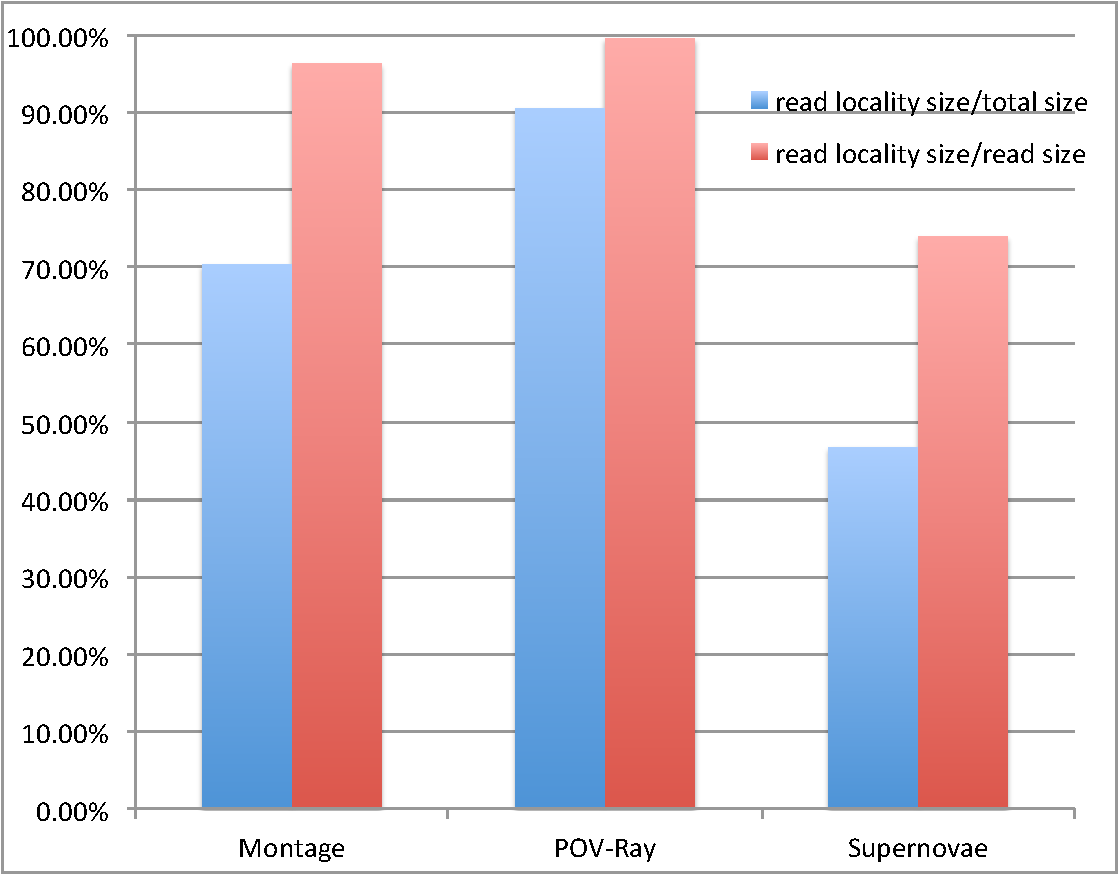
\includegraphics[width=8cm]{img/data_locality.pdf}
\caption{Data Locality}
\label{background:data locality}
\end{figure}

Since applications I/O pattern will affect the performance gains by using our propose architecture
greatly, We measure the I/O pattern for the applications shown in Table~.\ref{background:work flow
applications}.
We count the duplicated read at the same position and all write as data locality size, since all
these cases data can be read from or write to buffer.
Figure~.\ref{background:data locality} shows the results of these three applications. we can see
that the I/O pattern of all the three applications shows a strong data locality. Montage and Pov ray
are over 90\% and supernovae achieved over 80\%.

%The reason is that these applications are work flow application, the whole job consists of several
%sub jobs, the output of previous job can be the input of subsequent job, also some job will access
%the same input file.
%So if we buffer the output data and input data, the subsequent job can access the data via LAN.